\documentclass[12pt,fleqn]{article}

\usepackage[english]{babel}
\usepackage{SpeedyGonzales}
\usepackage{MediocreMike}
\usepackage{Blastoise}

\usepackage[backend=biber, style=alphabetic, citestyle=alphabetic, maxcitenames=4, maxbibnames=4, mincitenames=2]{biblatex}

\title{Synthesising Abstract Deep Computer Vision Pretraining Data}

\author{Søren Winkel Holm, s183911}
\date{\today}

\pagestyle{fancy}
\fancyhf{}
\lhead{02561 Computer Graphics}
\chead{}
\rhead{Technical University of Denmark}
\lfoot{Final Project: Synthetic Computer Vision Data}
\rfoot{Page \thepage{} of \pageref{LastPage}}

\graphicspath{{imgs/}}
\linespread{1.15}
\addbibresource{references.bib}

\begin{document}

\maketitle
\thispagestyle{fancy}
\tableofcontents
\newpage

%https://cocodataset.org/#detection-2016
%https://github.com/pytorch/vision/blob/main/references/segmentation/train.py

\section{Introduction}%
\label{sec:intro}
In the field of computer vision, deep learning is often used to solve problems such as object detection and image segmentation. Two main problems are (1) the high cost of annotating the image by producing the label maps (such as this) (2) the high cost of training the deep learning models. Automatic generation of scenes with corresponding label maps might be usable even if the scenes are abstract. Such data could be used to pretrain the deep learning model and act as an inductive bias such that less training and less data is required when actually training on the real dataset. For this to work, the generated scenes should have objects with object having some assigned class which determines some visual characteristics of the object. The scenes do not have to have anything to do with the actural task but need to make the model learn som basics of object detection, classification and segmentation. An easy first solution would be having the class determine the colour of the object but it is much more realistic if the objects are textured with noise functions and the parameters of the procedurally generated noise were determined by the class.

\section{Methods}%
\label{sec:method}
\subsection{Synthetic Scene Rendering}
\paragraph{Task 1: Noise Functions and The Simple Scene}
In the fragment shader, two noise functions were implemented, both accepting three-dimensional vector input.
\begin{enumerate}
    \item Improved Perlin noise (PN) using a permutation polynomial as \citeauthor{mcewan2012efficient} \cite{mcewan2012efficient}. 3D PN chooses pseudo-random gradients $\in \RR^3$ at regular grid points in each axis, interpolating a smooth function consistent with the gradients \cite{gustavson2005simplex}. 
    \item Sparse convolution noise (SC) as \citeauthor{frisvad2007fast} \cite{frisvad2007fast}. SC targets minimal artifacts or patterns by approximates the computationally expensive white noise filtered with a Gaussian kernel using a cubic kernel instead.
\end{enumerate}
Changing magnitude of the input vector -- the point at which the noise landscape is queried -- is equivalent to controlling the zoom level of the noise texture.
The implementations were largely based on reference implementations \cite{frisvad2016exploring}:
Only minor code changes and commenting were performed along with using the functions to texture the scene objects with a given noise scale $r$.

An initial scene was constructed by rendering a coloured sphere through 5-fold recursive subdivision of tetrahedra.
The sphere was shaded using Phong shading from a positional light behind a perspective camera.
The sphere was textured using the noise functions evaluated at normals scaled with a free parameter called noise scale.
This texturing was perform by letting the noise intensity controlling the diffuse light intensity, see Listing \ref{lst:light}.

Behind the sphere, a 2D noise textured background in black and white was placed.

The resulting scene can bee seen at Figure \ref{fig:t1} and the noise function and other variables can be user controlled on Page \href{file:///home/sorenmulli/Nextcloud/cand2/computer-graphics/afl/webgl-site/t1.html}{t1.html}.
\lstinputlisting[language=C, firstline=134, lastline=146, caption=Fragment shader snippet related to texturing of foreground objects, label=lst:light]{../webgl-site/t1.html}

\paragraph{Task 2: Random Scenes}
The simple scene was extended to rendering multiple spheres.
To generate a scene, the number of spheres to generate $1 \le N \le 20 $ and the background noise scale $r_\text{background} \in [1, 20]$ were randomly, uniformly chosen.
For each of the $N$ spheres, the scale, $(x, y)$-position and a number of lighting parameters were randomly chosen; see Listing \ref{lst:sphere}.

The randomly generated scenes can be seen and sphere variables controlled on Page \href{file:///home/sorenmulli/Nextcloud/cand2/computer-graphics/afl/webgl-site/t2.html}{t2.html}.
\lstinputlisting[language=Javascript, firstline=36, lastline=44, caption=Javascript code snippet with random variable generation run for each sphere, label=lst:sphere]{../webgl-site/randomness.js}
\paragraph{Task 3: Object Classes}
Three characteristics of each object were not set by the random scene and are instead set based on object class
\begin{itemize}
    \item Colour Hue $h \in [0, 360]$. The colour 
    \item Sphere elongation $\rho \in [0, 1]$
    \item Noise scale $r > 1$ used for the object
\end{itemize}

Choose a number of classes (maybe 3) and give each class a distribution of shapes, of colours and a distribution of noise parameters (such as related smoothing and scale). Assign each sphere to a class and let its shape, colour and noise be sampled from the class prior. (I will be using spheres and for shape I will use a model matrix that transforms the sphere into an ellipsoid by stretching it. The amount of stretching should thus be determined by object class)
\paragraph{Task 4: The Full Scene With Label Maps}
Add the possibility of producing the label image by having a rendering mode which does not have any lighting or texturing, just colours each object according to its class. This image will then have the class in the pixel position according to the object at that pixel position. Allow for saving the current canvas to a png.
\paragraph{Generated Datasets}


\subsection{Deep Image Segmentation}
\paragraph{Baseline Learning Task}
\paragraph{Addition of Synthetic Pretraining Data}

\section{Results}%
\label{sec:results}
\begin{figure}[H]
    \centering
        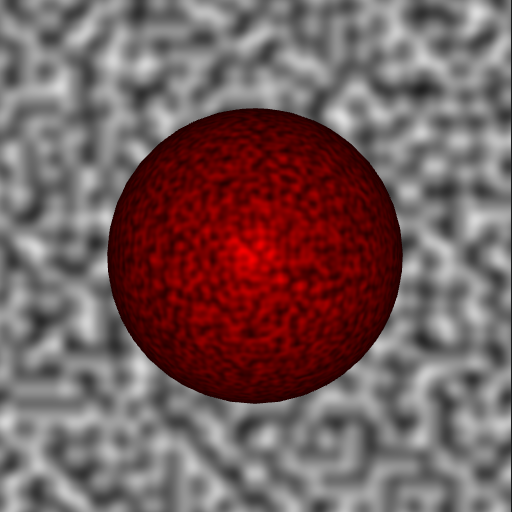
\includegraphics[width=.48\linewidth]{t1-perlin}
        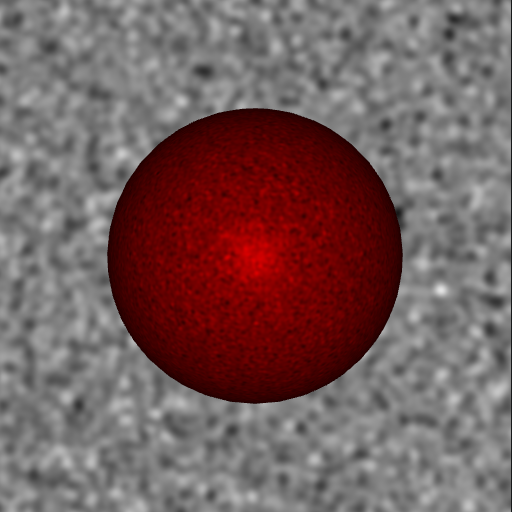
\includegraphics[width=.48\linewidth]{t1-sc}
    \caption{
        The Task 1 image where the scene is textured using PN (left) and SC (right); both with a noise scale of 25.
    }
    \label{fig:t1}
\end{figure}\noindent

\begin{figure}[H]
    \centering
        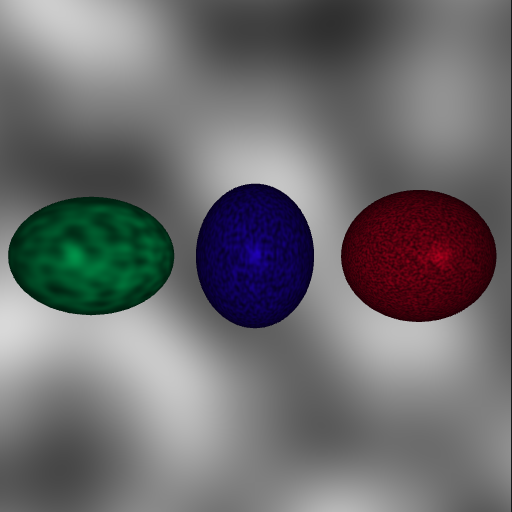
\includegraphics[width=.48\linewidth]{t3-avg-perlin}
        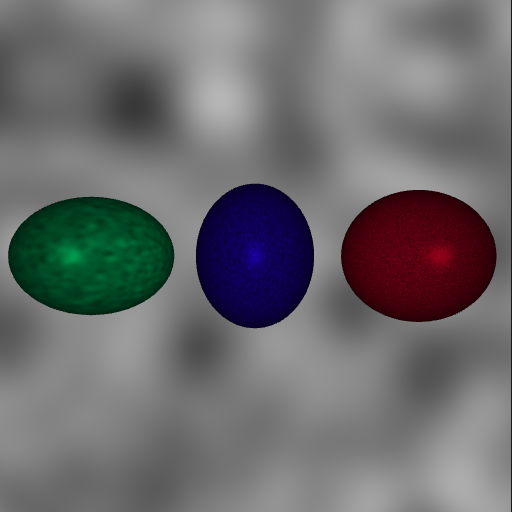
\includegraphics[width=.48\linewidth]{t3-avg-sc}
    \caption{
       Task 3 images showing the class prototype for each class from left to right in both PN (left) and SC (right).
       These spheres thus have their elongation $\rho$, noise scale $r$ and hue $h$ set to the class averages.
       To see examples of variation within classes, see Appendix \ref{sec:cls}.
    }
    \label{fig:t3}
\end{figure}\noindent

\section{Discussion}%
\label{sec:disc}
\begin{enumerate}
    \item Powerful benchmark for different methods generalization towards different difficulties: Explainability
\end{enumerate}

\clearpage

\printbibliography[heading=bibintoc]

\clearpage

\appendix
\section{Class examples}\label{sec:cls}
See Figure \ref{fig:t3-rand-perlin} for four random instances of object classes using PN and Figure \ref{fig:t3-rand-sc} for the same using SC.
\begin{figure}[H]
    \centering
        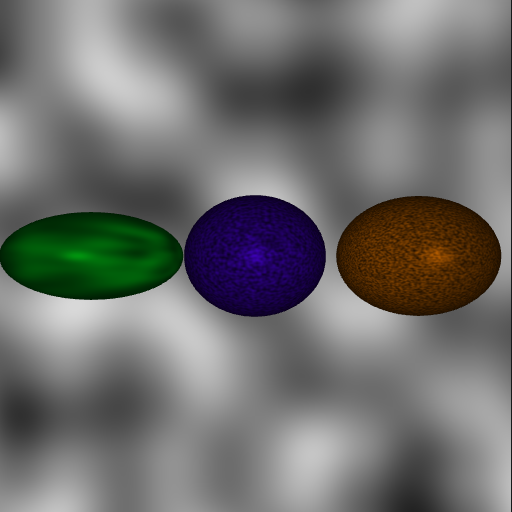
\includegraphics[width=.49\linewidth]{t3-rand1-perlin}
        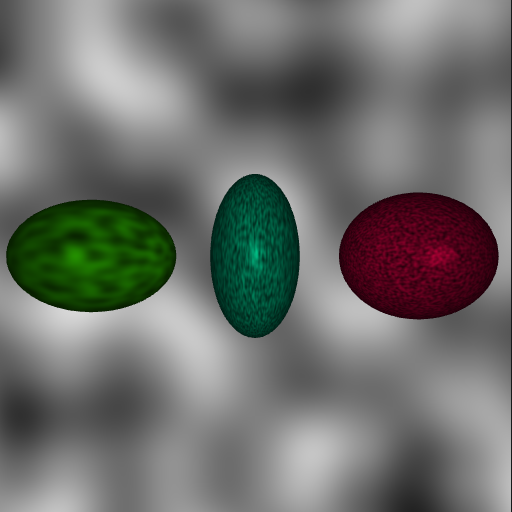
\includegraphics[width=.49\linewidth]{t3-rand2-perlin}
        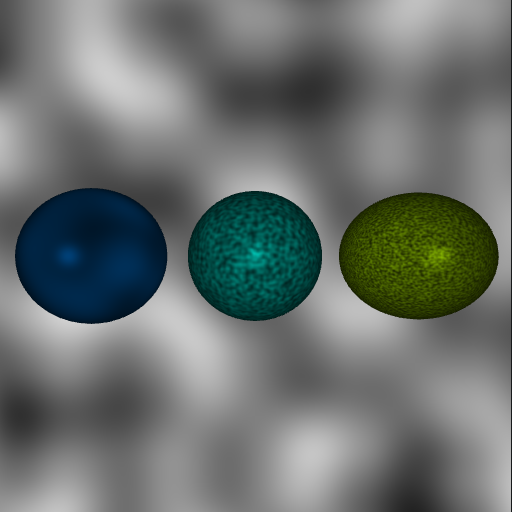
\includegraphics[width=.49\linewidth]{t3-rand3-perlin}
        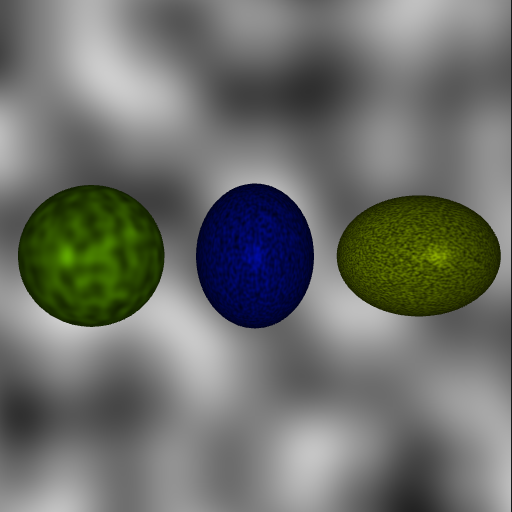
\includegraphics[width=.49\linewidth]{t3-rand4-perlin}
    \caption{
        Random instances of classes 1, 2, 3 textured using PN.
    }
    \label{fig:t3-rand-perlin}
\end{figure}\noindent

\begin{figure}[H]
    \centering
        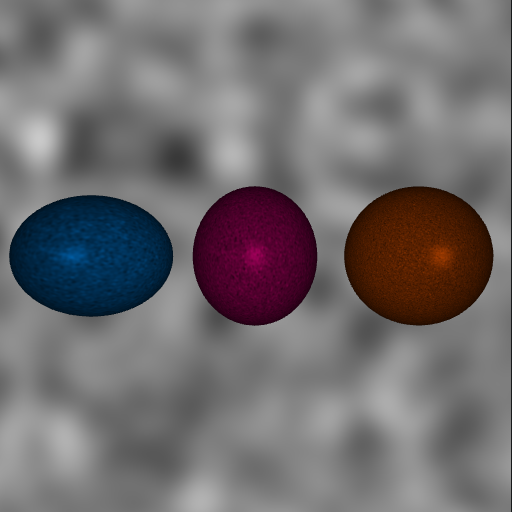
\includegraphics[width=.49\linewidth]{t3-rand1-sc}
        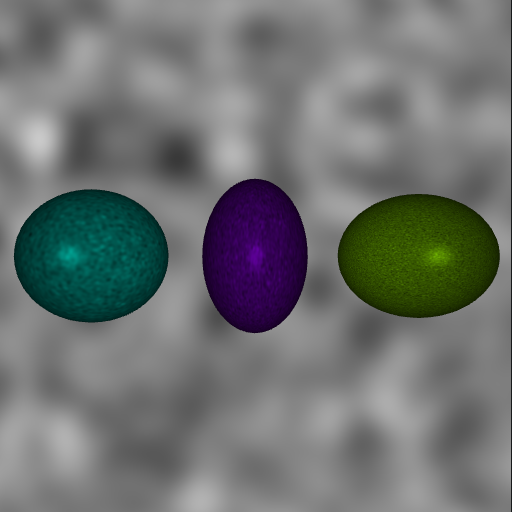
\includegraphics[width=.49\linewidth]{t3-rand2-sc}
        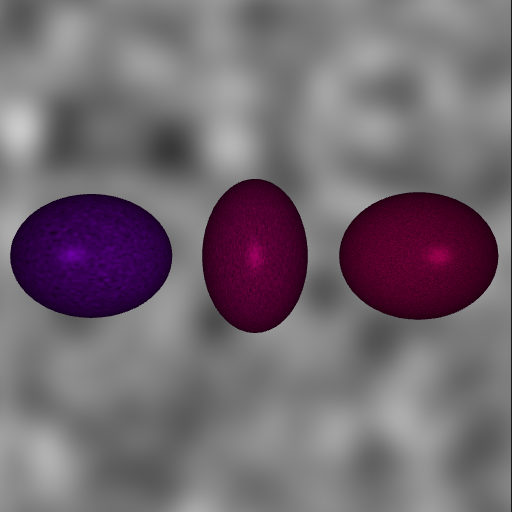
\includegraphics[width=.49\linewidth]{t3-rand3-sc}
        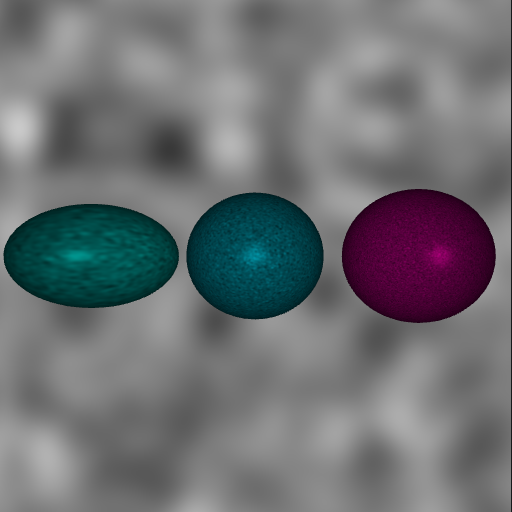
\includegraphics[width=.49\linewidth]{t3-rand4-sc}
    \caption{
        Random instances of classes 1, 2, 3 textured using SC.
    }
    \label{fig:t3-rand-sc}
\end{figure}\noindent


\end{document}

